\chapter{Introdução}

Desde a década de 60, robôs tem sido utilizados em ambientes indústriais. Manipuladores robóticos foram capazes de aumentar a produtividade, a eficiência e garantir um maior controle de qualidade dos processos. Além de serem capazes de realizar tarefas repetitivas em uma linha de montagem, muitos manipuladores o fazem com maior precisão e rapidez que um ser humano. 

Recentemente além de linhas de produção da industria, a robótica tem encontrado aplicação em instalações \textit{offshore} de óleo e gás. É de grande interesse utilizá-los para realizar tarefas onde a presença humana torna-se difícil, arriscada ou até mesmo impossível. Muitas empresas já tem utilizado soluções automatizadas tanto em ambientes submersos quanto acima do nível do mar. Braços robóticos tem sido de grande importância para executar tarefas que exigem interação mais complexa com o ambiente. Com isso em mente, foi desenvolvido um manipulador leve para o DORIS, robô guiado por trilhos para monitoração, inspeção e supervisão de ambientes não submersos de plataformas de petróleo \cite{xaud2016doris}.

\section{DORIS}
O uso de robôs em uma instalação de óleo e gás tem diversas vantagens. Pode reduzir o custo com manutenção de diversos sensores ao longo instalação e substituir humanos na realização de tarefas repetitivas, especialmente aquelas realizadas em ambientes perigosos, confinados ou prejudiciais a saúde. 

O projeto DORIS, desenvolvido pelo laboratório LEAD-GSCAR, da Universidade Federal do Rio de Janeiro, introduz um sistema robótico onde vagões guiados por trilhos carregam diversas câmeras, sensores e dispositivos para monitorar e inspecionar diferentes áreas e equipamento na parte \textit{topside} de plataformas.

As tarefas desse robô consistem principalmente em: monitorar perfis de temperatura utilizando câmeras térmicas infravermelhas, supervisão de pessoal não autorizado, detecção de anomalias sonoras utilizando microfones, detecção de vazamentos de gás com sensores de hidrocarbonetos, inspeção de padrões de vibração de maquinário crítico, interação com interfaces touchscreen na plataforma, processamento de dados coletados, armazenamento e transmissão de áudio e vídeo em tempo real.

A interação com o robô é feita através de um software chamado de RobotGUI, também desenvolvido pela equipe do LEAD-GSCAR. Através dele o operador é capaz de visualizar dados dos diversos sensores, reproduzir a transmissão de áudio e vídeo, enviar comandos de controle e configurar parâmetros, através de uma interface gráfica customizável. 

\begin{figure}[!ht]
\centering
  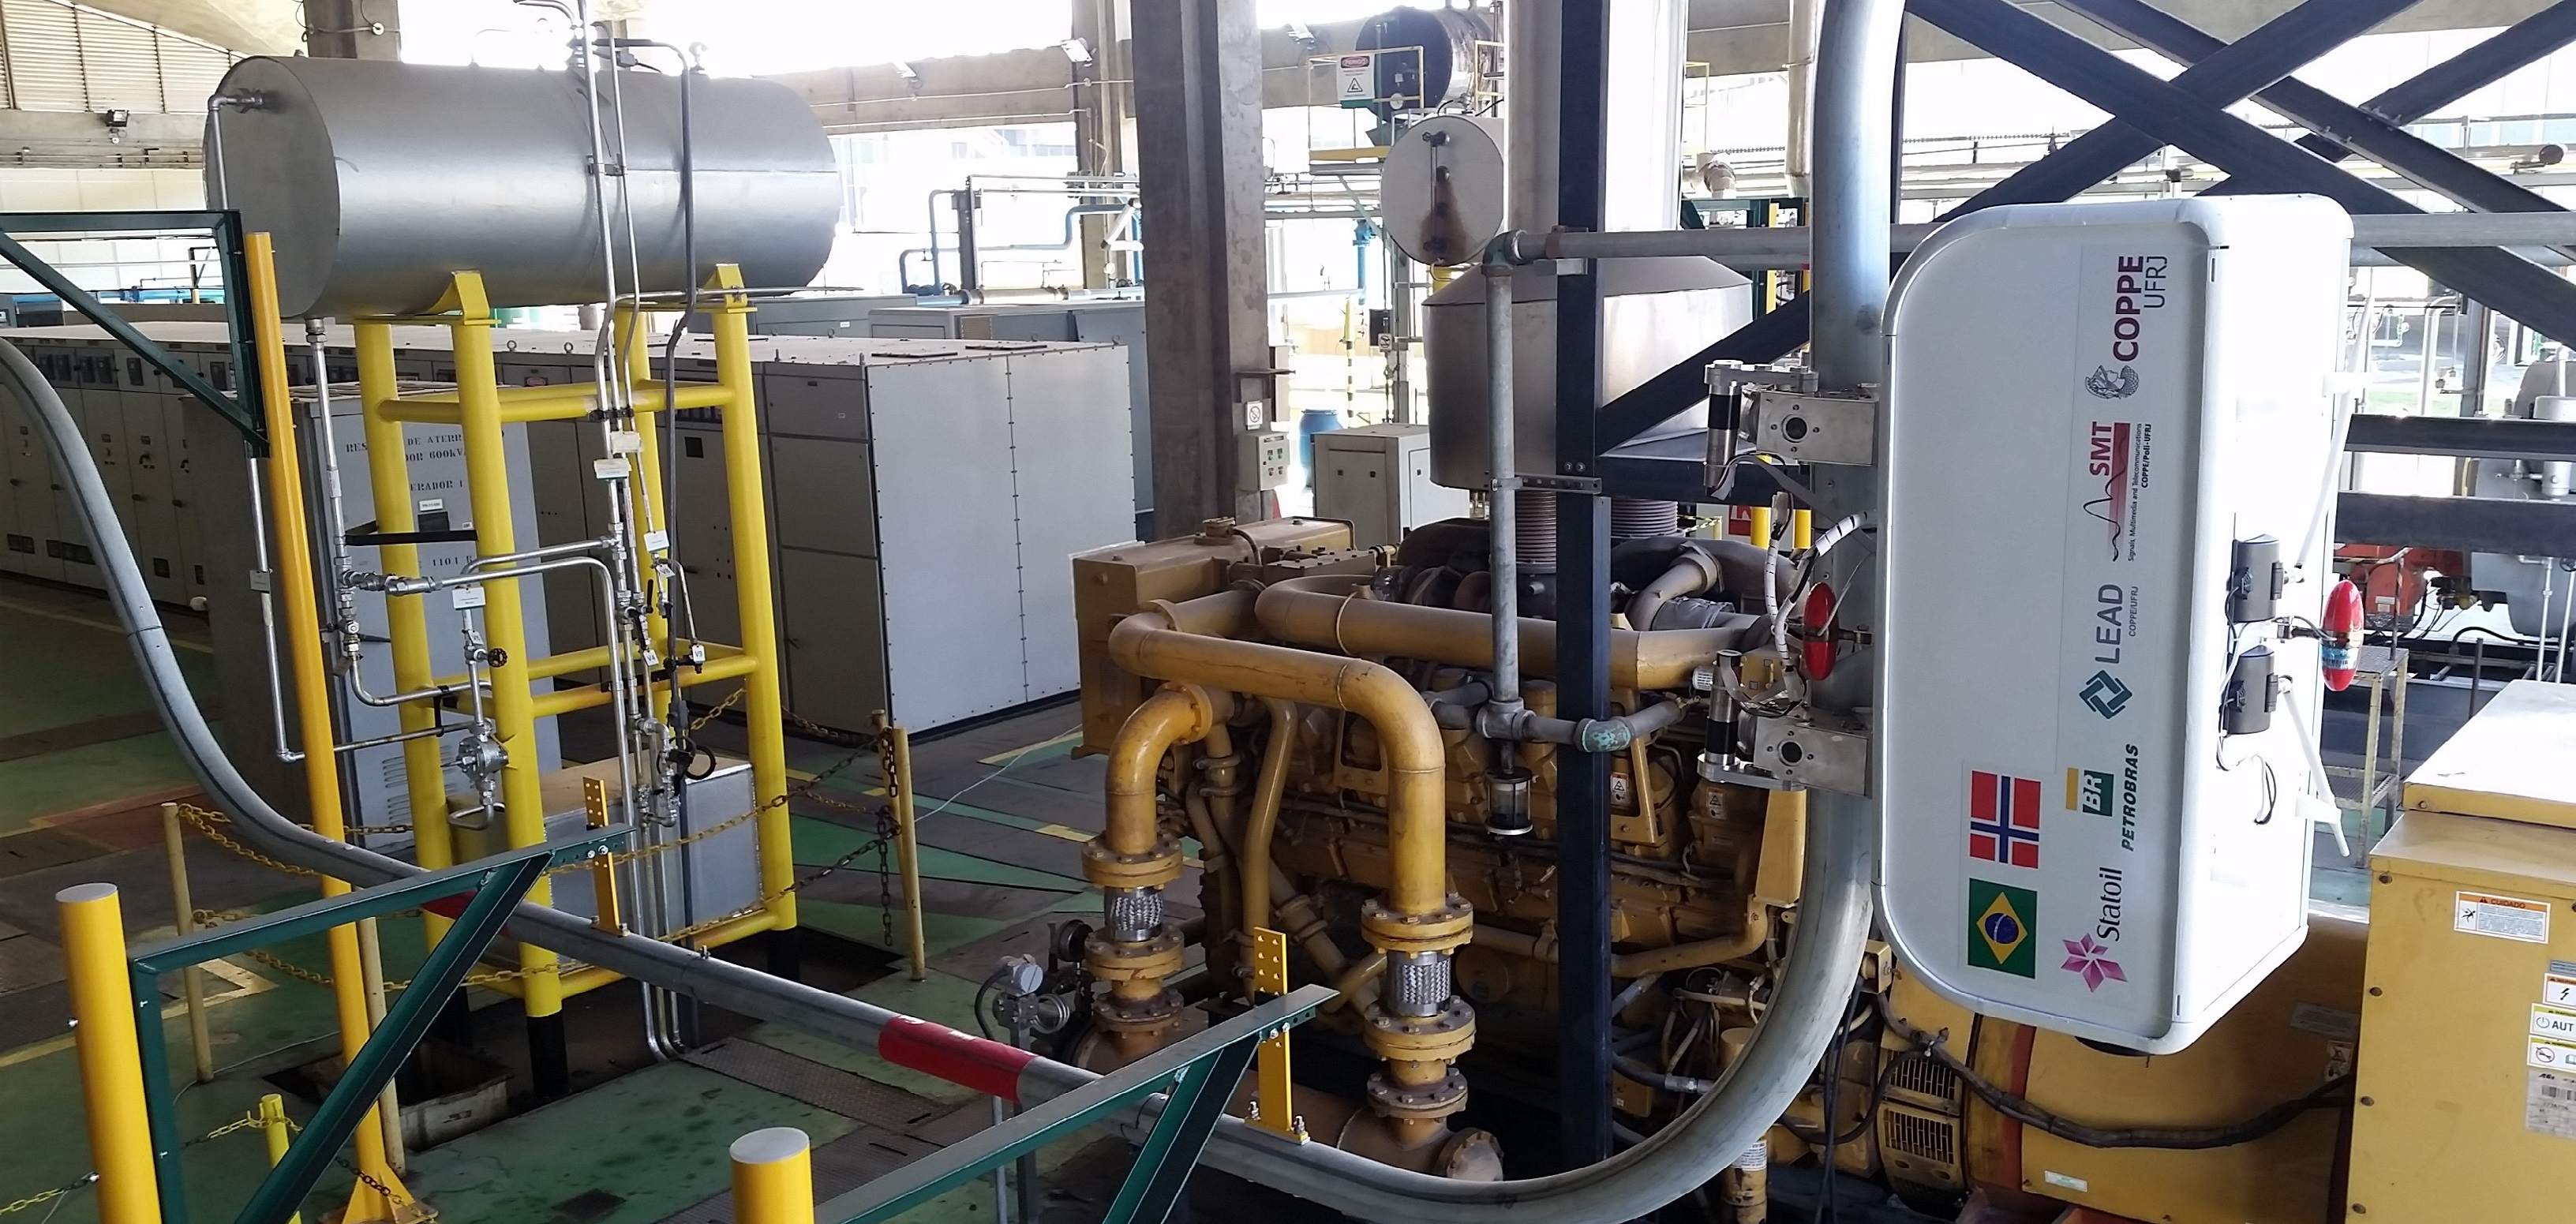
\includegraphics[width=\linewidth]{./img/cenpes_field.jpg}
  \caption{DORIS em operação no CENPES}
  \label{fig:cenpes_doris}
\end{figure}%

\section{Manipulador DORIS}
Considerando as tarefas mencionadas foi proposta a adição de um manipulador leve, de modo a extender o espaço de trabalho do robô. Com esse manipulador, pretende-se solucionar os problemas de
\begin{itemize}
\item mover a câmera acoplada ao efetuador, de modo a posicioná-la melhor ao longo da instalação
\item posicionar um sensor de vibração corretamente sobre a superfície de um equipamento na plataforma
\item interagir com \textit{touchscreens}
\end{itemize}

Foi dado a esse manipulador o nome TETIS. O projeto mecânico permite que ele assuma configurações de juntas diferentes, como mostra a figura (TODO). 

\section{ROS}
Com sua primeira versão em 2007, o \textit{framework} ROS (Robot Operating System) tem ganhado grande aceitação da comunidade na construção de aplicações para robôs. Consiste em um conjunto de bibliotecas e ferramentas que auxiliam desenvolvimento de software para robótica. Essa não é uma tarefa simples, pois o cada vez mais o escopo dos projetos aumenta, englobando algoritmos de controle, visão computacional, percepção e tomada de decisão.
 %em projetos de robótica.
Dentre as principais filosofias adotadas, destaca-se a modularidade. 
Muitos projetos tem a tendência de englobar código específico para o robô em questão, de modo que torna-se difícil reaproveitar algorítimos úteis. O ROS encoraja a comunidade de contribuidores a desenvolver pacotes que possam ser reutilizados em outros projetos.  

Processos que utilizam ROS são chamados de nós e comunicam entre si através de uma topologia ponto-a-ponto, podendo ser executados na mesma máquina ou em diferentes computadores em uma LAN. Dessa forma, os diferentes componentes necessários para o software de um robô podem ser encapsulados em nós, o que garante uma maior possibilidade de reaproveitamento, facilidade de alteração e versatilidade de execução.

\section{Motivação}
Com o projeto mecânico do manipulador finalizado, segue a etapa de modelagem e implementação de estratégias de controle. 
Nesse contexto, insere-se esse trabalho. Utilizando uma configuração alternativa do manipulador, mostrada na figura \ref{fig:tetis2} busca-se:
\begin{itemize}
\item Modelar e implementar estratégias de controle. %de posição, rastreamento de trajetória.

\item Realizar a integração com o RobotGUI, que já interage com os outros dispositivos do DORIS. O uso ROS proporciona uma maior versatilidade e facilidade para incorporação de novas funcionalidades, em comparação com abordagens tradicionais.

\item Utilizar a câmera para controle por servo visão onde o alvo é um marcador na forma de um QR Code em algum ponto de interesse, como por exemplo uma máquina a ser inspecionada. 

\item Utilizando \textit{Julia Language} permitir que o algoritmo de controle seja modificado em tempo de execução.
\end{itemize}


\section{Organização do trabalho}

No primeiro capítulo o trabalho foi contextualizado, descrevendo os objetivos do projeto DORIS e de seu manipulador TETIS. No segundo capítulo são mostrados conceitos de robótica necessários para a modelagem e controle de manipuladores robóticos. No capítulo 3 esses conceitos são aplicados ao manipulador TETIS. No capítulo 4 são abordados detalhes das ferramentas e da arquitetura utilizada para a implementação do software. No capítulo 5, são mostrados e discutidos os resultados dos testes dos diferentes modos de controle implementados. Por último, no capítulo 6 são apresentadas as conclusões sobre o trabalho e pontos para serem abordados em trabalhos futuros.